%% LyX 2.0.3 created this file.  For more info, see http://www.lyx.org/.
%% Do not edit unless you really know what you are doing.
\documentclass[twoside,english]{paper}
\usepackage{lmodern}
\renewcommand{\ttdefault}{lmodern}
\usepackage[T1]{fontenc}
\usepackage[latin9]{inputenc}
\usepackage[a4paper]{geometry}
\geometry{verbose,tmargin=3cm,bmargin=2.5cm,lmargin=2cm,rmargin=2cm}
\usepackage{color}
\usepackage{babel}
\usepackage{float}
\usepackage{bm}
\usepackage{amsthm}
\usepackage{amsmath}
\usepackage{amssymb}
\usepackage{graphicx}
\usepackage{esint}
\usepackage[unicode=true,pdfusetitle,
 bookmarks=true,bookmarksnumbered=false,bookmarksopen=false,
 breaklinks=false,pdfborder={0 0 0},backref=false,colorlinks=false]
 {hyperref}
\usepackage{breakurl}
\usepackage{makeidx}

\makeatletter

%%%%%%%%%%%%%%%%%%%%%%%%%%%%%% LyX specific LaTeX commands.
%% Because html converters don't know tabularnewline
\providecommand{\tabularnewline}{\\}

%%%%%%%%%%%%%%%%%%%%%%%%%%%%%% Textclass specific LaTeX commands.
\numberwithin{equation}{section}
\numberwithin{figure}{section}

%%%%%%%%%%%%%%%%%%%%%%%%%%%%%% User specified LaTeX commands.
\usepackage{babel}

\@ifundefined{showcaptionsetup}{}{%
 \PassOptionsToPackage{caption=false}{subfig}}
\usepackage{subfig}
\makeatother

\usepackage{listings}

\begin{document}

\title{Statistics}

\maketitle

\tableofcontents{}

\vspace{20pt}

{\tt APFEL++} is often used to fit non-perturbative functions, such as
parton distribution functions (PDFs) and fragmentation functions
(FFs), to experimental data. As a consequence, it is necessary to make
full use of the appropriate statistical tools that allow for a correct
treatment of the experimental information when comparing predictions
to data. This section is devoted to a detailed discussion of the
concepts and tools that are often used when fitting PDFs and FFs to
data.

Most of these tools are not directly implemented in {\tt APFEL++} but
can be found in other codes, as for instance {\tt NangaParbat} (see
https://github.com/vbertone/NangaParbat).

\section{The $\chi^2$ in the presence of correlations}

Suppose to have an ensamble of $n$ measurements having the following
structure:
\begin{equation}
  m_i\pm \sigma_{i,\rm stat} \pm \sigma_{i,\rm unc} \pm \sigma_{i,\rm
    corr}^{(1)}\pm\dots \pm \sigma_{i,\rm
    corr}^{(k)}\,,
\end{equation}
where $m_i$, with $i=1,\dots, n$, is the central value of the $i$-th
measurement, $\sigma_{i,\rm stat}$ its (uncorrelated) statistical
uncertainty, $\sigma_{i,\rm unc}$ its uncorrelated systematic
uncertainty\footnote{There could be more than one uncorrelated
  systematic uncertainty. In this case, $\sigma_{i,\rm unc}$ is just
  the square root of the sum in quadrature of all the uncorrelated
  systematic uncertainties.}, and $\sigma_{i,\rm corr}^{(l)}$, with
$l=1,\dots,k$, its correlated systematic uncertainties. With this
information at hand, one can construct the full covariance matrix
$V_{ij}$ as follows (see for example Ref.~\cite{Ball:2012wy}):
\begin{equation}
  V_{ij}=\left(\sigma_{i,\rm stat}^2 +\sigma_{i,\rm unc}^2\right)\delta_{ij} + \sum_{l=1}^{k}\sigma_{i,\rm
    corr}^{(l)}\sigma_{j,\rm
    corr}^{(l)}\,.
\label{eq:covmat}
\end{equation}
This is a clearly symmetric matrix. Given a set of predictions $t_i$
corresponding to the $n$ measurements of the ensamble, the $\chi^2$
takes the form:
\begin{equation}
  \chi^2=
  \sum_{i,j=1}^{n}\left(m_i-t_i\right)V_{ij}^{-1}\left(m_j-t_j\right) =
  \mathbf{y}^{T} \cdot \mathbf{V}^{-1} \cdot \mathbf{y}\,,
\label{eq:chi2cov}
\end{equation}
where in the second equality I have used the matricial notation and
defined $y_i = m_i-t_i$. A convenient way to compute the $\chi^2$
relies on the Cholesky decomposition of the covariance matrix
$\mathbf{V}$. In particular, it can be proven that any symmetric and
positive definite matrix $\mathbf{V}$ can be decomposed as:
\begin{equation}
\mathbf{V} = \mathbf{L}\cdot\mathbf{L}^{T}\,,
\label{eq:choleskydec}
\end{equation}
where $\mathbf{L}$ is a lower triangular matrix whose entries are
related recursively to those of $\mathbf{V}$ as follows:
\begin{equation}
\begin{array}{rcl}
  L_{kk} &=&\displaystyle \sqrt{V_{kk}-\sum_{j=1}^{k-1}L_{kj}^2}\,,\\
  \\
  L_{ik} &=&\displaystyle
             \frac{1}{L_{kk}}\left(V_{ik}-\sum_{j=1}^{k-1}L_{ij}L_{kj}\right)\,,\quad
             k < i\,,\\
\\
  L_{ik} &=&\displaystyle 0\,,\quad
             k > i\,.\\
\end{array}
\label{eq:cholalg}
\end{equation}
It is then easy to see that the $\chi^2$ can be written as:
\begin{equation}
\chi^2 = \left|\mathbf{L}^{-1}\cdot \mathbf{y}\right|^2\,.
\end{equation}
But the vector ${\bm \chi} \equiv \mathbf{L}^{-1}\cdot \mathbf{y}$ is
the solution of the linear system:
\begin{equation}
  \mathbf{L} \cdot {\bm \chi} = \mathbf{y}\,,
\label{eq:chivdef}
\end{equation}
that can be efficiently solved by forward substitution, so that:
\begin{equation}
  \chi^2 = \left|{\bm \chi}\right|^2\,.
\end{equation}
Following this procedure, one does not need to compute explicitly the
inverse of the covariance matrix $\mathbf{V}$, simplifying
significantly the computation of the $\chi^2$.

\section{Additive and multiplicative uncertainties}

The correlated systematic uncertainties $\sigma_{i,\rm corr}^{(l)}$
may be either \textit{additive} or \textit{multiplicative}. The nature
of the single uncertainties is typically provided by the experiments
that release the measurements. A typical example of multiplicative
uncertainty is the luminosity uncertainty but there can be others.

Now let us express all the correlated systematic uncertainties
$\sigma_{i,\rm corr}^{(l)}$ as relative to the associate central value
$m_i$, so that one defines\footnote{Note that this redefinition does
  not change the nature of the uncertainties, additive uncertainties
  remain additive as well as multiplicative uncertainties remain
  multiplicative.}:
\begin{equation}
\sigma_{i,\rm corr}^{(l)}\equiv  \delta_{i,\rm corr}^{(l)} m_i
\end{equation}
and let us also define
$s_i^2\equiv \sigma_{i,\rm stat}^2 +\sigma_{i,\rm unc}^2$ so that
Eq.~(\ref{eq:covmat}) can be rewritten as:
\begin{equation}
  V_{ij}=s_i^2\delta_{ij} + \left(\sum_{l=1}^{k}\delta_{i,\rm
    corr}^{(l)}\delta_{j,\rm
    corr}^{(l)}\right)m_im_j\,.
\label{eq:covmat2}
\end{equation}
Now I split the correlated systematic uncertainties into $k_a$
additive uncertainties and $k_m$ multiplicative uncertainties, such
that $k_a+k_m=k$. This way Eq.~(\ref{eq:covmat2}) takes the form:
\begin{equation}
  V_{ij}=s_i^2\delta_{ij} + \left(\sum_{l=1}^{k_a}\delta_{i,\rm
    add}^{(l)}\delta_{j,\rm
    add}^{(l)}+\sum_{l=1}^{k_m}\delta_{i,\rm
    mult}^{(l)}\delta_{j,\rm
    mult}^{(l)}\right)m_im_j\,.
\label{eq:covmat3}
\end{equation}
It is believed that this definition of the covariance matrix is
problematic in that it results in the so-called D'Agostini bias of the
multiplicative uncertainties~\cite{DAgostini:1993arp}. A possible
solution to this problem is the so-called
$t_0$-prescription~\cite{Ball:2009qv}, where the experimental central
value $m_i$ in the multiplicative term is replaced by a fixed
theoretical predictions $t_i^{(0)}$, typically computed in a previous
fit in which the ``standard'' definition of the covariance matrix in
Eq.~(\ref{eq:covmat}) (often referred to as \textit{experimental}
definition) is used. Applying the $t_0$ prescription, the covariance
matrix takes the form:
\begin{equation}
  V_{ij}=s_i^2\delta_{ij} + \sum_{l=1}^{k_a}\delta_{i,\rm
    add}^{(l)}\delta_{j,\rm
    add}^{(l)}m_im_j+\sum_{l=1}^{k_m}\delta_{i,\rm
    mult}^{(l)}\delta_{j,\rm
    mult}^{(l)}t_i^{(0)}t_j^{(0)}\,.
\label{eq:covmat4}
\end{equation}

% \section{Artificial generation of correlated systematics}

% In order to implement the definition of the $\chi^2$ discussed above,
% it is necessary to have the experimental information in terms of the
% correlated systematic uncertainties $\sigma_{i,\rm corr}^{(l)}$. This
% is what the experimental collaborations usually release. However, in
% some cases this information is given in terms of a covariance
% matrix. Therefore, one needs to find a workaround to generate
% correlated systematic uncertainties out of a covariance matrix. 

% Given a $n \times n$ symmetric matrix $\mathbf{C}$, it will have $n$
% orthonormal eigenvectors $\mathbf{x}^{(i)}$, such that
% $\mathbf{x}^{(i)}\cdot \mathbf{x}^{(j)}=\delta_{ij}$, each of which
% will have a non-negative eigenvalue $\lambda_i$ associated:
% \begin{equation}
%   \mathbf{C}\cdot \mathbf{x}^{(i)} = \lambda_i \mathbf{x}^{(i)}\,, \quad
%   i =1,\dots,n\,.
% \end{equation}
% If one defines:
% \begin{equation}
%   \sigma_{i,\rm corr}^{(l)} = \sqrt{\lambda_l} x_i^{(l)}\,,\quad
%   i,l=1,\dots,n\,,
% \label{eq:artsys}
% \end{equation}
% one can show that:
% \begin{equation}
%   \sum_{l=1}^{n}\sigma_{i,\rm corr}^{(l)}\sigma_{j,\rm corr}^{(l)}
%   =C_{ij}\,.
% \label{eq:artsydef}
% \end{equation}
% To prove this equality, I start from the following matricial relation:
% \begin{equation}
% \mathbf{C} =\mathbf{Q}\cdot \mathbf{\Lambda}\cdot \mathbf{Q}^{-1}\,,
% \end{equation}
% where $\mathbf{\Lambda}$ is a diagonal matrix with the eigenvalues
% $\lambda_i$ on the diagonal ($\Lambda_{ij} = \lambda_i\delta_{ij}$),
% while $\mathbf{Q}$ is a matrix whose columns are the eigenvectors
% $\mathbf{x}^{(i)}$ ($Q_{ij} = x_{i}^{(j)}$). In addition, since in
% this particular case
% $\mathbf{x}^{(i)}\cdot \mathbf{x}^{(j)}=\delta_{ij}$, this implies
% that:
% \begin{equation}
% \mathbf{Q}^T \cdot \mathbf{Q}  = \mathbf{I}\quad\Rightarrow\quad
% \mathbf{Q}^{-1} =  \mathbf{Q}^{T}\,,
% \end{equation}
% so that:
% \begin{equation}
%   \mathbf{C} =\mathbf{Q}\cdot \mathbf{\Lambda}\cdot
%   \mathbf{Q}^{T}\,.
% \label{eq:diagC}
% \end{equation}
% It follows that:
% \begin{equation}
%   C_{ij} =\sum_{k,l=1}^{n}Q_{ik}\Lambda_{kl} Q_{jl} = \sum_{k,l=1}^{n} x_{i}^{(k)}
%   \lambda_{k}\delta_{kl}x_{j}^{(l)} = \sum_{l=1}^{n} \lambda_{l}x_{i}^{(l)}
%   x_{j}^{(l)}=\sum_{l=1}^{n}\sigma_{i,\rm corr}^{(l)}\sigma_{j,\rm corr}^{(l)} \,,
% \end{equation}
% as required.

% The matrix \textbf{C} can be regarded as the correlated contribution to
% the full covariance matrix \textbf{V}. In particular, considering
% Eqs.~(\ref{eq:covmat}) and~(\ref{eq:covmat2}), one can write:
% \begin{equation}
% \mathbf{V} = \mathbf{U} + \mathbf{C}\,,
% \end{equation}
% where $\mathbf{U}$ is a diagonal matrix of uncorrelated uncertainties:
% \begin{equation}
% U_{ij} = s_i^2\delta_{ij}\,.
% \end{equation}
% This defines the matrix $\mathbf{C}$ as:
% \label{eq:corrdef}
% \begin{equation}
% \mathbf{C} = \mathbf{V} - \mathbf{U}\,,
% \end{equation}
% such that, given a $n\times n$ covariance matrix $\mathbf{V}$ along
% with its uncorrelated contribution $\mathbf{U}$, one can generate a
% set of $n$ \textit{artificial} correlated systematics according to
% Eq.~(\ref{eq:artsys}), where $\mathbf{C}$ is given in
% Eq.~(\ref{eq:corrdef}), for each of the $n$ measurements. This allows
% one to implement Eq.~(\ref{eq:covmat4}) for the construction of the
% covariance matrix.

\section{Determining the systematic shifts}\label{eq:sysshifts}

In order to visualise the effect of systematic uncertainties, it is
instructive to compute the \textit{systematic shift} generated by the
systematic uncertainties. To do so, one needs to write the $\chi^2$ in
terms of the so-called ``nuisance parameters'' $\lambda_\alpha$. One
can show that the definition of the $\chi^2$ in Eq.~(\ref{eq:chi2cov})
is equivalent to~\cite{Ball:2012wy}:
\begin{equation}
\chi^2 = \sum_{i=1}^n\frac{1}{s_i^2}\left(m_i -t_i
  -\sum_{\alpha=1}^k\lambda_\alpha \sigma_{i,\rm corr}^{(\alpha)}
\right)^2 + \sum_{\alpha=1}^k\lambda_\alpha^2\,.
\label{eq:chi2nuis}
\end{equation}
The optimal value of the nuisance parameters can be computed by
minimising the $\chi^2$ with respect to them, that is imposing:
\begin{equation}
\frac{\partial \chi^2}{\partial \lambda_\beta} = 0\,.
\end{equation}
This yields the system:
\begin{equation}
  \sum_{\beta=1}^kA_{\alpha\beta}\lambda_\beta =\rho_\alpha\,,
\label{eq:nuissys}
\end{equation}
with:
\begin{equation}
A_{\alpha\beta}= \delta_{\alpha\beta}+\sum_{i=1}^n\frac{\sigma_{i,\rm
    corr}^{(\alpha)}\sigma_{i,\rm
    corr}^{(\beta)}}{s_i^2}\quad\mbox{and}\quad
\rho_\alpha=\sum_{i=1}^n\frac{m_i-t_i}{s_i^2}\sigma_{i,\rm
  corr}^{(\alpha)}\,,
\label{eq:sysing}
\end{equation}
that determines the values of $\lambda_\beta$. The quantity:
\begin{equation}
d_i =\sum_{\alpha=1}^k\lambda_\alpha \sigma_{i,\rm corr}^{(\alpha)}
\end{equation}
in Eq.~(\ref{eq:chi2nuis}) can be interpreted as a shift caused by the
correlated systematic uncertainties. Defining the shifted predictions
as:
\begin{equation}
\overline{t}_i =t_i+d_i\,,
\end{equation}
the $\chi^2$ reads:
\begin{equation}
  \chi^2 = \sum_{i=1}^n\left(\frac{m_i -\overline{t}_i}{s_i}\right)^2
  + \sum_{\alpha=1}^k\lambda_\alpha^2\,.
\label{eq:chi2nuisshift}
\end{equation}
Therefore, up to a penalty term given by the sum of the square of the
nuisance parameters, the $\chi^2$ takes the form of the uncorrelated
definition. In order to achieve a visual assessment of the agreement
between data and theory, it appears natural to compare the central
experimental values $m_i$ to the shifted theoretical predictions
$\overline{t}_i$ in units of the uncorrelated uncertainty $s_i$.

\section{Effect of cuts on the $\chi^2$}

A relevant question to ask is what is the effect of possible cuts on
the input data set on the form of the $\chi^2$ in the presence of
correlations. In order to address this question, I consider a simple
data set made of two datapoints equipped with a single uncorrelated
uncertainty and a single fully-correlated uncertainty:\footnote{Note
  that one needs to include \textit{also} an uncorrelated uncertainty
  because otherwise the covariance matrix would be singular. This a
  symptom of the fact that if no uncorrelated uncertainties are
  present, the two points would be totally dependent on each
  other. This observation will be relevant in the following.}
\begin{equation}
S:\quad\{m_i\pm \sigma_i^u\pm \sigma_i^c\}\,,\quad i  =1,2\,.
\label{eq:fullset}
\end{equation}
The resulting covariance matrix reads:
\begin{equation}
\mathbf{V}=\begin{pmatrix}
(\sigma_1^u)^2+ (\sigma_1^c)^2 & \sigma_1^c \sigma_2^c \\
\sigma_1^c \sigma_2^c & (\sigma_2^u)^2+ (\sigma_2^c)^2
\end{pmatrix}\,,
\end{equation}
with inverse:
\begin{equation}
\mathbf{V}^{-1}=\frac{1}{(\sigma_1^u \sigma_2^u)^2+ (\sigma_1^c \sigma_2^u)^2+ (\sigma_1^u \sigma_2^c)^2}\begin{pmatrix}
(\sigma_2^u)^2+ (\sigma_2^c)^2 & -\sigma_1^c \sigma_2^c \\
-\sigma_1^c \sigma_2^c & (\sigma_1^u)^2+ (\sigma_1^c)^2
\end{pmatrix}\,.
\end{equation}
In addition, the set of two theoretical predictions $\{t_i\}$ that
allows one to define a column vector of residuals
$\mathbf{r}^{\rm T}=(r_1,\;r_2)$ with $r_i=m_i-t_i$. The $\chi^2$ then
takes the following explicit expression:
\begin{equation}
  \chi^2= \mathbf{r}^{\rm T}\cdot \mathbf{V}^{-1}\cdot \mathbf{r}=
  \frac{r_1^2\left[(\sigma_2^u)^2+
      (\sigma_2^c)^2\right]+r_2^2\left[(\sigma_1^u)^2+
      (\sigma_1^c)^2\right]-2 r_1 r_2\sigma_1^c
    \sigma_2^c}{(\sigma_1^u \sigma_2^u)^2+ (\sigma_1^c \sigma_2^u)^2+
    (\sigma_1^u \sigma_2^c)^2}\,.
\label{eq:fullchi2}
\end{equation}
Now, suppose one wants to exclude the datapoint with $i=2$ from the
definition of the $\chi^2$. The possibly most natural way to proceed
is to exclude the point, along with its uncertainties, directly from
the set in Eq.~(\ref{eq:fullset}). This straightforwardly leads to the
following $\chi^2$:
\begin{equation}
{\chi}_{\rm cut\;1}^2 = \frac{r_1^2}{(\sigma_1^u)^2+
  (\sigma_1^c)^2}\,.
\label{eq:redchi21}
\end{equation}
However, this procedure might be questioned in that it artificially
modifies the original data set by effectively defining a \textit{new}
data set where the point $i=2$ is not present. In the absence of
correlations this is a sound procedure because each single datapoint
can be regarder an independent subset of the original
set. However, this is not the case when correlations are present.

Therefore, it is necessary to devise a method that avoids any
modification of the data set but yet allows one to prevent specific
datapoints to contribute to the $\chi^2$. In general, the purpose of
excluding datapoints from a fit is to avoid that the model used to
compute the predictions is forced outside its application region. One
can therefore \textit{enforce} that the model exactly agrees with the
datapoints to be excluded. This effectively amounts to set $t_2=m_2$,
or equivalently $r_2=0$, reducing Eq.~(\ref{eq:fullchi2}) to:
\begin{equation}
  \chi_{\rm cut\;2}^2= 
  \frac{r_1^2\left[(\sigma_2^u)^2+ (\sigma_2^c)^2\right]}{(\sigma_1^u
    \sigma_2^u)^2+ (\sigma_1^c \sigma_2^u)^2+ (\sigma_1^u
    \sigma_2^c)^2}\,.
\label{eq:fullchi2trunc}
\end{equation}
This has the clear advantage that the experimental information,
including correlations, remains totally intact. In order to show that
Eq.~(\ref{eq:fullchi2trunc}) has the right properties, I first take
the limit for $\sigma_2^c\rightarrow 0$. This gives:
\begin{equation}
  \lim_{\sigma_2^c\rightarrow 0}\chi_{\rm cut}^2= 
  \frac{r_1^2}{(\sigma_1^u)^2+ (\sigma_1^c)^2}\,,
\end{equation}
which reproduces the result of Eq.~(\ref{eq:redchi21}). This was to be
expected because no reference to the point $i=2$ can remain after the
removal of its correlation to the point $i=1$. In addition, it is also
very instructive to take the limit $\sigma_2^u\rightarrow 0$
Eq.~(\ref{eq:fullchi2trunc}), which gives:
\begin{equation}
\lim_{\sigma_2^u\rightarrow 0}\chi_{\rm cut}^2= 
\frac{r_1^2}{ (\sigma_1^u)^2}\,.
\end{equation}
In this case, not only any reference to the point $i=2$ drops out, but
also the dependence of the $\chi^2$ on the correlation uncertainty of
the point $i=1$ disappears. Despite at first sight this looks
counterintuitive, it seems to be the correct behaviour. To see this,
observe that, if the point $i=2$ has no uncorrelated uncertainty, its
fluctuations are totally driven by the fluctuations of the point
$i=1$. Therefore, the point $i=2$ is completely dependent on the point
$i=1$ and thus cannot give any contribution to the $\chi^2$. In
addition, the correlation uncertainty of the point $i=1$ must also be
irrelevant because, being $i=2$ totally correlated to $i=1$, any
correlation of $i=1$ to $i=2$ translates into a correlation to itself
and this cannot contribute to the $\chi^2$ either. Importantly, if one
takes the limit $\sigma_1^u\rightarrow 0$, the $\chi^2$ diverges no
matter the value of $\sigma_1^c$. This is consistent with setting
$\sigma_1^u=\sigma_2^u$ since the beginning in Eq.~(\ref{eq:fullset})
which indeed gives a singular $\chi^2$ because the covariance matrix
is singular. Eq.~(\ref{eq:redchi21}) does not produce these features
hanging in favour of Eq.~(\ref{eq:fullchi2trunc}).

As a further argument in favour of Eq.~(\ref{eq:fullchi2trunc}) and
against Eq.~(\ref{eq:redchi21}), I consider a larger data set with,
say, $n$ data points and split it into two subsets with $n_1$ and
$n_2$ data points, respectively, such that $n_1+n_2=n$. As I will
explicitly show below, Eq.~(\ref{eq:fullchi2trunc}) guarantees that
the $\chi^2$'s of the two subsets, $\chi_1^2$ and $\chi_2^2$, combine
sensibly to give the total $\chi^2$. I will also show that this is not
the case for Eq.~(\ref{eq:redchi21}). The fulfilment of this condition
is crucial to ensure that the experimental information carried by the
data set as a whole is preserved also when one is either not able or
does not want to make predictions for subset of data points. This
property is particularly relevant in fits that adopt the
cross-validation method as stopping criterion. In this context, the
full data set is indeed split into a training subset and a validation
subset and only the $\chi^2$ of the training set is minimised while
the validation $\chi^2$ is monitored. Since the cross-validation
method relies on the exploitation of the full experimental information
to stop the fit, it is necessary that training and validation
$\chi^2$'s combine meaningfully.

Now, I move to explicitly show that the generalisation of
Eq.~(\ref{eq:fullchi2trunc}) to an $n$-point data set where $n_2$ are
cut away and $n_1$ remain fulfils the requirement:
\begin{equation}
  \chi^2 = \left|{\bm \chi}_1+{\bm \chi}_2\right|^2\,,
\label{eq:compisition1}
\end{equation}
where the vectors ${\bm \chi}_1$ and ${\bm \chi}_2$ are defined
according to Eq.~(\ref{eq:chivdef}). To define them more precisely,
without loss of generality, one can order the data points in such a
way that those labelled with $i=1,\dots,n_1$ belong to the first
subset and the points labelled with $i=n_1+1,\dots,n_1+n_2(=n)$ belong
to the second subset. The entries of the ${\bm \chi}_1$ and ${\bm \chi}_2$ are then given by:
\begin{equation}
\bm \chi_{1,k} = \sum_{j=1}^{n_1} L_{kj}^{-1}y_j\,,\quad\mbox{and}\quad
\bm \chi_{2,k} = \sum_{j=n_1+1}^{n} L_{kj}^{-1}y_j\,,
\end{equation}
where $L_{ij}^{-1}$ are the entries of the inverse of the Cholesky
decomposition $\mathbf{L}$ of the covariance $\mathbf{V}$. It should
be clear that, according to the generalisation of the prescription of
Eq.~(\ref{eq:fullchi2trunc}), one has:
\begin{equation}
\chi_1^2= \left|\bm \chi_{1}\right|^2\,,\quad\mbox{and}\quad \chi_2^2= \left|\bm \chi_{2}\right|^2\,.
\end{equation}
The proof of Eq.~(\ref{eq:compisition1}) runs as follows:
\begin{equation}
\begin{array}{rcl}
  \chi^2 &=&\displaystyle 
             \sum_{i=1}^n\sum_{j=1}^nr_iV_{ij}^{-1}r_j=\sum_{i=1}^{n_1}\sum_{j=1}^{n_1}r_iV_{ij}^{-1}r_j
             + \sum_{i=n_1+1}^{n}\sum_{j=n_1+1}^{n}r_iV_{ij}^{-1}r_j+2
             \sum_{i=1}^{n_1}\sum_{j=n_1+1}^{n}r_iV_{ij}^{-1}r_j\\
  \\
         &=& \displaystyle \sum_{k=1}^{n}\left(\sum_{i=1}^{n_1}L^{-1}_{ki}r_i\right)\left(\sum_{j=1}^{n_1}L^{-1}_{kj}r_j\right)
             +
             \sum_{k=1}^{n}\left(\sum_{i=n_1+1}^{n}L^{-1}_{ki}r_i\right)\left(\sum_{j=n_1+1}^{n}L^{-1}_{kj}r_j\right)\\
\\
 &+&\displaystyle 2
             \sum_{k=1}^n\left(\sum_{i=1}^{n_1}L_{ki}^{-1}r_i\right)\left(\sum_{j=n_1+1}^{n}L_{kj}^{-1}r_j\right)\\
  \\
         &=&\displaystyle {\bm \chi}_1^{\rm T}\cdot{\bm \chi}_1+{\bm \chi}_2^{\rm T}\cdot{\bm \chi}_2 +2
             {\bm \chi}_1^{\rm T}\cdot{\bm \chi}_2 =\left|{\bm \chi}_1+{\bm \chi}_2\right|^2\,,
\end{array}
\label{eq:combinechi2s}
\end{equation}
where in the last step of the first line I have used the fact that the
covariance matrix (and thus its inverse) is symmetric upon exchange of
the indices while in the second and third lines I have used the
Cholesky decomposition of the covariance matrix. It straightforward to
see that Eq.~(\ref{eq:redchi21}) does not fulfils the same
relation. The fact that Eq.~(\ref{eq:compisition1}) is consistent with
how the $\chi^2$'s should combine can be better seen by giving it a
geometrical interpretation.

\subsection{A geometrical point of view}

It is instructive to consider the question of cuts from a geometrical
point of view. In fact, the whole bunch of questions related to the
computation of the $\chi^2$ can be nicely visualised as a set of
geometrical operations in a multidimensional space $\mathcal{M}$
(manifold) equipped with the appropriate metric tensor. Based on the
definition in Eq.~(\ref{eq:chi2cov}), the $\chi^2$ can be interpreted
as the squared absolute value of the $n$-dimensional vector
$\mathbf{y}$ given by the difference between the vector of
experimental central values $\mathbf{m}$ and the vector of theoretical
predictions $\mathbf{t}$. Importantly, the scalar product required to
compute this absolute value has to be computed using the inverse of
the covariance matrix $\mathbf{V}^{-1}$ as a covariant
positive-definite metric tensor.\footnote{The contravariant
  counterpart of $\mathbf{V}^{-1}$ is clearly $\mathbf{V}$, given that
  $\mathbf{V}^{-1}\cdot\mathbf{V}=\mathbb{I}$.} Borrowing the Einstein
notation to represent scalar products, \textit{i.e.} defining
contravariant vectors with upper index as:
\begin{equation}
y^i = V^{-1}_{ij}y_j\,,
\end{equation}
where the sum over $j$ between 1 and $n$ is understood, the $\chi^2$ is
the \textit{norm} squared of the vector $\mathbf{y}$ in the space
$\mathcal{M}$.
\begin{equation}
  \chi^2 = \mathbf{y}^{\rm T}\cdot \mathbf{V}^{-1}\cdot \mathbf{y} =
  y^iy_i\equiv \left\|\mathbf{y}\right\|^2\,.
\end{equation}
It is interesting to notice that the minimisation of the $\chi^2$ can
then be regarded as the attempt to align the vector $\mathbf{t}$ to
the vector $\mathbf{m}$ in the space $\mathcal{M}$ in such a way that
their difference is as small as possible.

The enforcement of cuts can be accommodated in this framework by
requiring that the $\chi^2$ is the squared absolute value (or length)
of the projection of $\mathbf{y}$ in the subspace of $\mathcal{M}$,
$\mathcal{M}_{1}$, defined by the components of the vector
$\mathbf{m}$ corresponding to the points that pass the
cut. Introducing the operator $\mathbf{P}$ that projects any vector in
$\mathcal{M}$ onto $\mathcal{M}_{1}$, the corresponding $\chi^2$ will
read:
\begin{equation}
  \chi^2_{1} = \left(\mathbf{P}\cdot \mathbf{y}\right)^{\rm T}\cdot \mathbf{V}^{-1}\cdot \left(\mathbf{P}\cdot \mathbf{y}\right)=\left(\mathbf{P}\cdot \mathbf{y}\right)^i \left(\mathbf{P}\cdot \mathbf{y}\right)_i=\left\|\mathbf{P}\cdot\mathbf{y}\right\|^2\,.
\end{equation}
The matrix corresponding to the projector $\mathbf{P}$ is simply the
diagonal matrix with zero's and one's on the diagonal depending on
whether the point is excluded or included,
respectively.\footnote{Notice that $\mathbf{P}$ is indeed idempotent,
  \textit{i.e.} $\mathbf{P}^2=\mathbf{P}$, as required.} The net
effect of the projector $\mathbf{P}$ is to set to zero the components
of the vector of residuals $\mathbf{y}$ corresponding to the points
excluded by the cut. This is in agreement with
Eq.~(\ref{eq:fullchi2trunc}) in the case of a two-dimensional space.

It is interesting to define the projector
$\mathbf{Q}=\mathbb{I}-\mathbf{P}$ orthogonal to
$\mathbf{P}$\footnote{$\mathbf{Q}$ is such that
  $\mathbf{Q}^2=\mathbf{Q}$, $\mathbf{P}\cdot\mathbf{Q}=0$, and
  $\mathbf{P}+\mathbf{Q}=\mathbb{I}$.} such that the corresponding
$\chi^2$ reads:
\begin{equation}
  \chi^2_{2} = \left(\mathbf{Q}\cdot \mathbf{y}\right)^{\rm T}\cdot \mathbf{V}^{-1}\cdot \left(\mathbf{Q}\cdot \mathbf{y}\right) =\left(\mathbf{Q}\cdot \mathbf{y}\right)^i \left(\mathbf{Q}\cdot \mathbf{y}\right)_i =\left\|\mathbf{Q}\cdot\mathbf{y}\right\|^2\,.
\end{equation}
With these definitions at hands, one can write the total $\chi^2$ as:
\begin{equation}
  \chi^2= \left\|\mathbf{y}\right\|^2 = \left\|\mathbf{P}\cdot\mathbf{y}+\mathbf{Q}\cdot\mathbf{y}\right\|^2 = \chi^2_{1} + \chi^2_{2} + 2 \left(\mathbf{P}\cdot \mathbf{y}\right)^i \left(\mathbf{Q}\cdot \mathbf{y}\right)_i\,.
\end{equation}
that agrees with Eq.~(\ref{eq:combinechi2s}). In conclusion, the
introduction of a cut on the full data set has a nice geometrical
interpretation: the resulting $\chi^2$ corresponds to the norm of the
projection of the vector or residual $\mathbf{y}$, defined on the
manifold $\mathcal{M}$ with covariant metric $\mathbf{V}^{-1}$, on to
the subspace $\mathcal{M}_1$ defined by the projector
$\mathbf{P}$. This is consistent with Eq.~(\ref{eq:compisition1}) and
provides it with a nice geometrical interpretation.\footnote{As an
  interesting aside, the difference between the following equalities:
$$
\chi^2 = \left|\mathbf{L}^{-1}\cdot
  \mathbf{y}\right|^2\quad\mbox{and}\quad \chi^2= \left\|\mathbf{y}\right\|^2\,,
$$
can be paralleled with the norm of a vector in special relativity in
the Euclidean space in the first case (where the time component is
multiplied by the imaginary unit $i$ and the space components are left
unchanged) and in Minkowski space in the second case. Indeed, the
Cholesky decomposition of the metric tensor
$g_{\mu\nu}=\mbox{diag}(-1,1,1,1)$ is
$L_{\mu\nu}=\mbox{diag}(i,1,1,1)$.}

\section{Monte Carlo replica generation}

In this section, I consider the Monte Carlo generation of artificial
replicas. The aim is to obtain a formula for the generation of
replicas that gives rise to a figure of merit distributed correctly,
\textit{i.e.} that follows a $\chi^2$ distribution with as many
degrees of freedom as number of data points. Following
Ref.~\cite{wiki:xxx}, one requires that the $\chi^2$, that in
matricial form can be expressed as:
\begin{equation}
  \chi^2 = \mathbf{y}^{T}\cdot \mathbf{V}^{-1} \cdot \mathbf{y}\,,
\label{eq:chi2matrix}
\end{equation}
where $\mathbf{V}$ is the $n\times n$ covariance matrix, being $n$ the
number of datapoints, and $\mathbf{y}$ is a column vector with $n$
entries that can be expressed as:
\begin{equation}
y_j = f_j-m_j\,,
\end{equation}
with $m_j$ a given value (to be thought as the central value) and
$f_j$ its fluctuated value, is distributed like:
\begin{equation}
\chi^2\sim \sum_{i=1}^{n}z_i^2=|\mathbf{z}|^2\,,
\label{eq:wikipedia}
\end{equation}
where $z_1,\dots , z_n$ are independent, standard normal random
variables, \textit{i.e.} such that:
\begin{equation}
\langle z_i\rangle=0\quad\mbox{and}\quad \langle z_iz_j\rangle =
\delta_{ij}\,,
\label{eq:averages}
\end{equation}
where the symbol $\langle\,\dots\rangle$ indicates the
average.\footnote{The relevant identities are:
\begin{equation}
  \langle z_i^{2n-1}\rangle = 0\quad\mbox{and}\quad \langle
  z_i^{2n}\rangle= (2n-1)!!\quad n=1,2,3,\dots\,,
\end{equation}
where $(2n-1)!!=1\cdot3\cdot\dots\cdot(2n-1)$ is the odd
semi-factorial. When considering combinations of two random variables
the result is:
\begin{equation}
  \langle z_i^n z_j^m\rangle = \left\{
\begin{array}{ll}
\langle z_i^{n+m}\rangle&\quad i = j\\
\langle z_i^n\rangle\langle z_j^m\rangle&\quad i \neq j
\end{array}
\right.
\end{equation}} This immediately tells that:
\begin{equation}
\langle\chi^2\rangle=n\,.
\end{equation}
As already discussed above, Eq.~(\ref{eq:chi2matrix}) can
alternatively be written as:
\begin{equation}
\chi^2 = \left|\mathbf{L}^{-1}\cdot \mathbf{y}\right|^2\,,
\label{explicitchi2chol}
\end{equation}
where $\mathbf{L}$ is the Cholesky decomposition of the matrix
$\mathbf{V}$, such that:
\begin{equation}
\mathbf{V} = \mathbf{L}\cdot\mathbf{L}^{T}\,.
\label{eq:choleskydecagain}
\end{equation}
Comparing Eqs.~(\ref{explicitchi2chol}) and~(\ref{eq:wikipedia}), one
can infer that the following relation should hold:
\begin{equation}
\mathbf{L}^{-1}\cdot \mathbf{y}\sim\mathbf{z}\,,
\end{equation}
which immediately implies:
\begin{equation}
\mathbf{y}\sim\mathbf{L}\cdot\mathbf{z}\,,
\end{equation}
or equivalently:
\begin{equation}
f_j\sim m_j+\sum_{i=1}^nL_{ji}z_i\,.
\label{eq:deviations}
\end{equation}
In conclusion, in order for the $\chi^2$ to have the correct
distribution, the fluctuations $f_j$ around the experimental central
values $m_j$ of a given Monte Carlo replica have to be computed
according to Eq.~(\ref{eq:deviations}).

I now show that Eq.~(\ref{eq:deviations}) reproduces the statistical
properties of the original ensamble of data. To do so, I compute
average and correlations of Eq.~(\ref{eq:deviations}) using
Eq.~(\ref{eq:averages}). The average gives:
\begin{equation}
\langle f_j\rangle = m_j+\sum_{i=1}^nL_{ji}\langle z_i \rangle = m_j\,,
\end{equation}
as expected. The correlation instead gives:
\begin{equation}
\begin{array}{rcl}
\langle f_j f_k\rangle &=& \displaystyle \left\langle
  \left(m_j+\sum_{i=1}^nL_{ji}z_i\right)
  \left(m_k+\sum_{i'=1}^nL_{ki'}z_{i'}\right)\right\rangle\\
\\
&=& \displaystyle m_jm_k+\sum_{i,i'=1}^nL_{ji'}L_{ki'}\langle z_{i'}
    z_{i'}\rangle=\langle f_j \rangle\langle f_k\rangle+V_{jk}\,,
\end{array}
\end{equation}
again as expected. These are fundamental requirements of a sound Monte
Carlo ensamble (see also Eq.~(10) of Ref.~\cite{Ball:2009qv}).

Eq.~(\ref{eq:deviations}) should be compared to the more ``standard''
Monte-Carlo replica generation formulas such as those given in
Refs.~\cite{Ball:2008by, Ball:2014uwa}. I now specifically consider
Eq.~(20) of Ref.~\cite{Ball:2014uwa} that I report here in terms of
relative uncertainties $\delta$'s matching our notation:
\begin{equation}
\widetilde{f}_j\sim m_j\prod_{m=1}^{k_m}\left(1+\delta_{{\rm mult},j}^{(m)} x_m\right)\left(1+\delta_{{\rm unc},j} z_j+\sum_{a=1}^{k_a} \delta_{{\rm add},j}^{(a)} y_a\right)\,,
\label{eq:nnpdfmc}
\end{equation}
where $z_j$, $y_a$, and $x_m$ are independent random variables. I now
expand the product in the front up to second order in $x$
\begin{equation}
  \prod_{m=1}^{k_m}\left(1+\delta_{{\rm mult},j}^{(m)}
    x_m\right)=1+\sum_{m=1}^{k_m}\delta_{{\rm mult},j}^{(m)}
  x_m+\sum_{m=1}^{k_m}\sum_{m'=1\atop m'\neq m}^{k_m}\delta_{{\rm
      mult},j}^{(m)}\delta_{{\rm mult},j}^{(m')}x_m x_{m'}+\mbox{trilinear}\,,
\end{equation}
where the ``trilinear'' corrections correspond to combinations of the
kind $x_ix_jx_k$, with $i\neq j\neq k\neq i$, such that their average
vanishes:
$\langle x_ix_jx_k\rangle = \langle x_i\rangle \langle x_j
\rangle\langle x_k\rangle = 0$. This allows one to expand
Eq.~(\ref{eq:nnpdfmc}) as:
\begin{equation}
\begin{array}{rcl}
\widetilde{f}_j&\sim&\displaystyle m_j\Bigg(1+\delta_{{\rm unc},j} z_j+\sum_{a=1}^{k_a} \delta_{{\rm add},j}^{(a)} y_a +\sum_{m=1}^{k_m}\delta_{{\rm mult},j}^{(m)}
  x_m\\
\\
&+&\displaystyle\delta_{{\rm unc},j} \sum_{m=1}^{k_m} \delta_{{\rm mult},j}^{(m)}
    z_jx_m+\sum_{a=1}^{k_a} \sum_{m=1}^{k_m}\delta_{{\rm add},j}^{(a)} \delta_{{\rm mult},j}^{(m)} y_a 
  x_m\\
\\
&+&\displaystyle \sum_{m=1}^{k_m}\sum_{m'=1\atop m'\neq m}^{k_m}\delta_{{\rm
      mult},j}^{(m)}\delta_{{\rm mult},j}^{(m')}x_m x_{m'}\Bigg)+\mbox{trilinear}\,.
\end{array}
\label{eq:nnpdfmcexp}
\end{equation}
Since Eq.~(\ref{eq:nnpdfmcexp}) involves only terms that have at most
one power of the same random variable, the average of
$\widetilde{f}_j$ automatically yields:
\begin{equation}
  \langle \widetilde {f}_j\rangle = m_j\,,
\label{eq:centralvaluenn}
\end{equation}
in agreement with the expectation. I now compute the correlations
making use of the combination rules of random variables. This gives:
\begin{equation}
\begin{array}{rcl}
  \langle \widetilde{f}_j \widetilde{f}_k\rangle&\sim&\displaystyle m_jm_k\Bigg(1+\delta_{{\rm unc},j}^2\delta_{jk}+\sum_{a=1}^{k_a} \delta_{{\rm add},j}^{(a)}\delta_{{\rm add},k}^{(a)} +\sum_{m=1}^{k_m}\delta_{{\rm mult},j}^{(m)}\delta_{{\rm mult},k}^{(m)}\\
\\
&+&\displaystyle\delta_{{\rm unc},j}^2 \sum_{m=1}^{k_m} \delta_{{\rm mult},j}^{(m)}\delta_{{\rm  mult},k}^{(m)}
  +\sum_{a=1}^{k_a} \sum_{m=1}^{k_m}\delta_{{\rm add},j}^{(a)}\delta_{{\rm add},k}^{(a)} \delta_{{\rm mult},j}^{(m)} \delta_{{\rm mult},k}^{(m)} \\
\\
&+&\displaystyle \sum_{m=1}^{k_m}\sum_{m'=1\atop m'\neq m}^{k_m}\delta_{{\rm
      mult},j}^{(m)}\delta_{{\rm
      mult},k}^{(m)}\delta_{{\rm mult},j}^{(m')}\delta_{{\rm
    mult},k}^{(m')}+\mathcal{O}(\delta^6)\Bigg)\\
\\
&=&\displaystyle \langle \widetilde{f}_j\rangle \langle
    \widetilde{f}_k\rangle +V_{jk}+\mathcal{O}(\sigma_{\rm mult}^2 s^2, \sigma_{\rm mult}^2 \sigma_{\rm add}^2)\,.
\end{array}
\label{eq:corrnn}
\end{equation}
In conclusion, Eq.~(\ref{eq:nnpdfmc}) reproduces exactly the central
values of the original ensemble (see Eq.~(\ref{eq:centralvaluenn}))
while it reproduces correlations only up to corrections proportional
to the fourth power of the typical uncertainty. Interestingly, these
corrections are all proportional to $\sigma_{\rm mult}^2$. This means
that, in the absence of multiplicative uncertainties, somewhat
expectedly Eq.~(\ref{eq:nnpdfmc}) \textit{exactly} reproduces the
correlations. On the other hand, if multiplicative uncertainties are
large these correction become potentially sizeable preventing
Eq.~(\ref{eq:nnpdfmc}) from correctly reproducing the correlations of
the original ensemble.

The case of Eq.~(13) of Ref.~\cite{Ball:2008by} is more involved
because of the presence of the square-root sign for the relative
multiplicative uncertainties. This case can be handled again be
expanding to second order the factor depending on multiplicative
uncertainties with the only difference that, due to the expansion:
\begin{equation}
  \sqrt{1+x}=1+\frac12x-\frac18x^2+\mathcal{O}(x^3)\,,
\end{equation}
the square root produces a factor $1/2$ in front of the linear terms
and a factor $-1/8$ in front of the quadratic terms. This is expected
to reduce the impact of the corrections terms in
Eq.~(\ref{eq:corrnn}).

It is instructive to work out whether Eq.~(\ref{eq:deviations}) can be
directly related to the Monte-Carlo replicas generation formulas given
in Refs.~\cite{Ball:2008by, Ball:2014uwa}. The aim is to find a
closed-form expression for the Cholesky-decomposition matrix
$\mathbf{L}$ of the covariance matrix $\mathbf{V}$ in terms of the
single uncertainties. Through Eq.~(\ref{eq:deviations}), this will
finally allow one to derive a formula of the same kind of those given
in Refs.~\cite{Ball:2008by, Ball:2014uwa}. The basic observation is
that the covariance matrix can be written as:
\begin{equation}
\mathbf{V} = \mathbf{D}+ \sum_{l=1}^k 
\mathbf{V}^{(l)} = \sum_{l=0}^k \mathbf{L}^{(l)}\cdot \mathbf{L}^{(l)T}\,,
\end{equation}
with:
\begin{equation}
L_{ij}^{(l)}=\left\{
\begin{array}{ll}
s_i\delta_{ij}&\quad l = 0\,,\\
\sigma_i^{(l)}\delta_{j1}&\quad 1\leq l\leq k\,.
\end{array}
\right.
\end{equation}
On the other hand, one also knows that:
\begin{equation}
  \mathbf{V} = \mathbf{L}\cdot \mathbf{L}^T\,,
\end{equation}
therefore:
\begin{equation}
  \mathbf{L}\cdot \mathbf{L}^T=\sum_{l=0}^k \mathbf{L}^{(l)}\cdot \mathbf{L}^{(l)T}\,.
\end{equation}
The question is to express $\mathbf{L}$ in terms of all the
$\mathbf{L}^{(l)}$. Unfortunately though this equation has no general
solution. However, a step forward can be done be exploiting the fact
that the matrices $\mathbf{V}^{(l)}$ are positive semidefinite
(\textit{i.e.} they have zero determinant) and thus their Cholesky
decomposition is not unique. In particular, provided that $k\leq n$,
one can choose:
\begin{equation}
\widetilde{L}_{ij}^{(l)}=
\sigma_i^{(l)}\delta_{jl}\,,\quad 1\leq l\leq k\leq n\,,
\end{equation}
such that:
\begin{equation}
  \left(\sum_{l=1}^k\widetilde{\mathbf{L}}^{(l)}\right)\cdot\left(
    \sum_{l'=1}^k\widetilde{\mathbf{L}}^{(l')}\right)=\sum_{l=1}^k 
  \mathbf{V}^{(l)}\,.
\label{eq:choldecomp2}
\end{equation}
However, choosing:
\begin{equation}
\widetilde{\mathbf{L}} = \mathbf{L}^{(0)} +
\sum_{l=1}^k\widetilde{\mathbf{L}}^{(l)}\,,
\label{eq:CholVapprox}
\end{equation}
and multiplying it for its transpose would give:
\begin{equation}
\widetilde{\mathbf{L}}\cdot \widetilde{\mathbf{L}}^T = \mathbf{V} + \sum_{l=1}^k\left(\mathbf{L}^{(0)}\cdot \widetilde{\mathbf{L}}^{(l)T}+\widetilde{\mathbf{L}}^{(l)}\cdot \mathbf{L}^{(0)T}\right)\,,
\end{equation}
that gives back the covariance matrix plus a spurious term. Writing
the expression above in terms of single entries, one finds:
\begin{equation}
\sum_{m=1}^n\widetilde{L}_{im}\widetilde{L}_{jm} = V_{ij} + s_i \sigma_{j}^{(i)}+s_j\sigma_{i}^{(j)}\,.
\end{equation}
The peculiarity here is that the upper index of $\sigma_{j}^{(i)}$ and
$\sigma_{i}^{(j)}$, since $k\leq n$ (and in fact usually $k\ll n$,
\textit{i.e.} the number of correlated uncertainties is typically much
smaller than the number of data points), exceeds the allowed range. To
fix this problem, I just assume $\sigma_{j}^{(i)}=0$ for $i>k$. This
finally gives:
\begin{equation}
\sum_{m=1}^n\widetilde{L}_{im}\widetilde{L}_{jm} = V_{ij}\,,\quad
\mbox{for } i,j>k\,,
\end{equation}
that means that, by adopting the Cholesky decomposition in
Eq.~(\ref{eq:choldecomp2}), part of the covariance matrix (usually the
largest part) is exactly recovered. Therefore,
$\widetilde{\mathbf{L}}$ Eq.~(\ref{eq:CholVapprox}) seems to be a
generally good approximator to the real Cholesky decomposition of the
covariance matrix $\mathbf{V}$. Plugging this equation into
Eq.~(\ref{eq:deviations}) immediately gives:
\begin{equation}
  f_j\sim m_j+z_js_j + \sum_{l=1}^{k}z_l \sigma_{j,\rm
    corr}^{(l)}\,.
\label{eq:deviations2}
\end{equation}
It is interesting to focus on similarities and differences with the
formulas present in the literature. I will specifically consider
Eq.~(13) of Ref.~\cite{Ball:2008by} and Eq.~(20) of
Ref.~\cite{Ball:2014uwa}.

Let us start by considering the case in which there are only
uncorrelated and correlated additive uncertainties. In this case,
Refs.~\cite{Ball:2008by, Ball:2014uwa} are in mutual agreement and
only in partial agreement with our Eq.~(\ref{eq:deviations2}), the
difference being that the random numbers used to generate the
fluctuation associated to the $k$ correlated uncertainties are equal
to the first $k$ of the $n$ used for the uncorrelated uncertainties
(remember the requirement $k\leq n$). Of course, if $k\ll n$, as it
often happens, the agreement between Eq.~(\ref{eq:deviations2}) and
Refs.~\cite{Ball:2008by, Ball:2014uwa} is asymptotically good.

When considering also correlated multiplicative uncertainties there
are differences across formulas of Refs.~\cite{Ball:2008by, Ball:2014uwa} and Eq.~(\ref{eq:deviations2}). While
Eq.~(\ref{eq:deviations2}) treats multiplicative uncertainties on the
same footing as additive uncertainties (consistently with the
construction of the covariance matrix in Eq.~(\ref{eq:covmat})),
Refs.~\cite{Ball:2008by, Ball:2014uwa} introduce a multiplicative
factor. In addition, Ref.~\cite{Ball:2008by} distinguishes between
relative and absolute multiplicative uncertainties.
\begin{figure}[h]
  \begin{centering}
    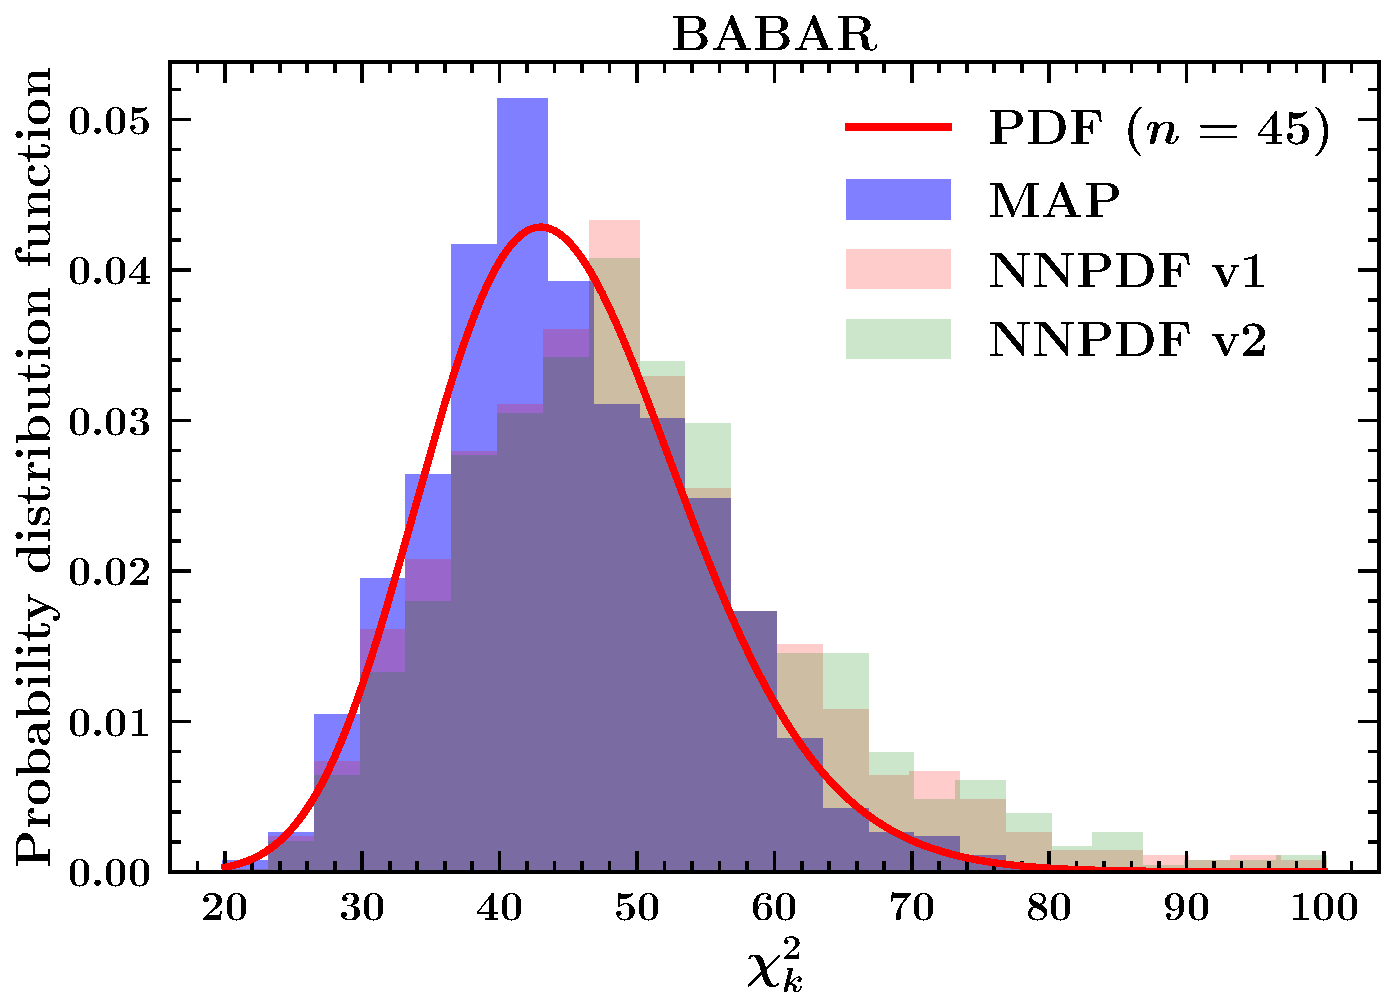
\includegraphics[width=0.49\textwidth]{plots/Chi2DistBABAR.pdf}
    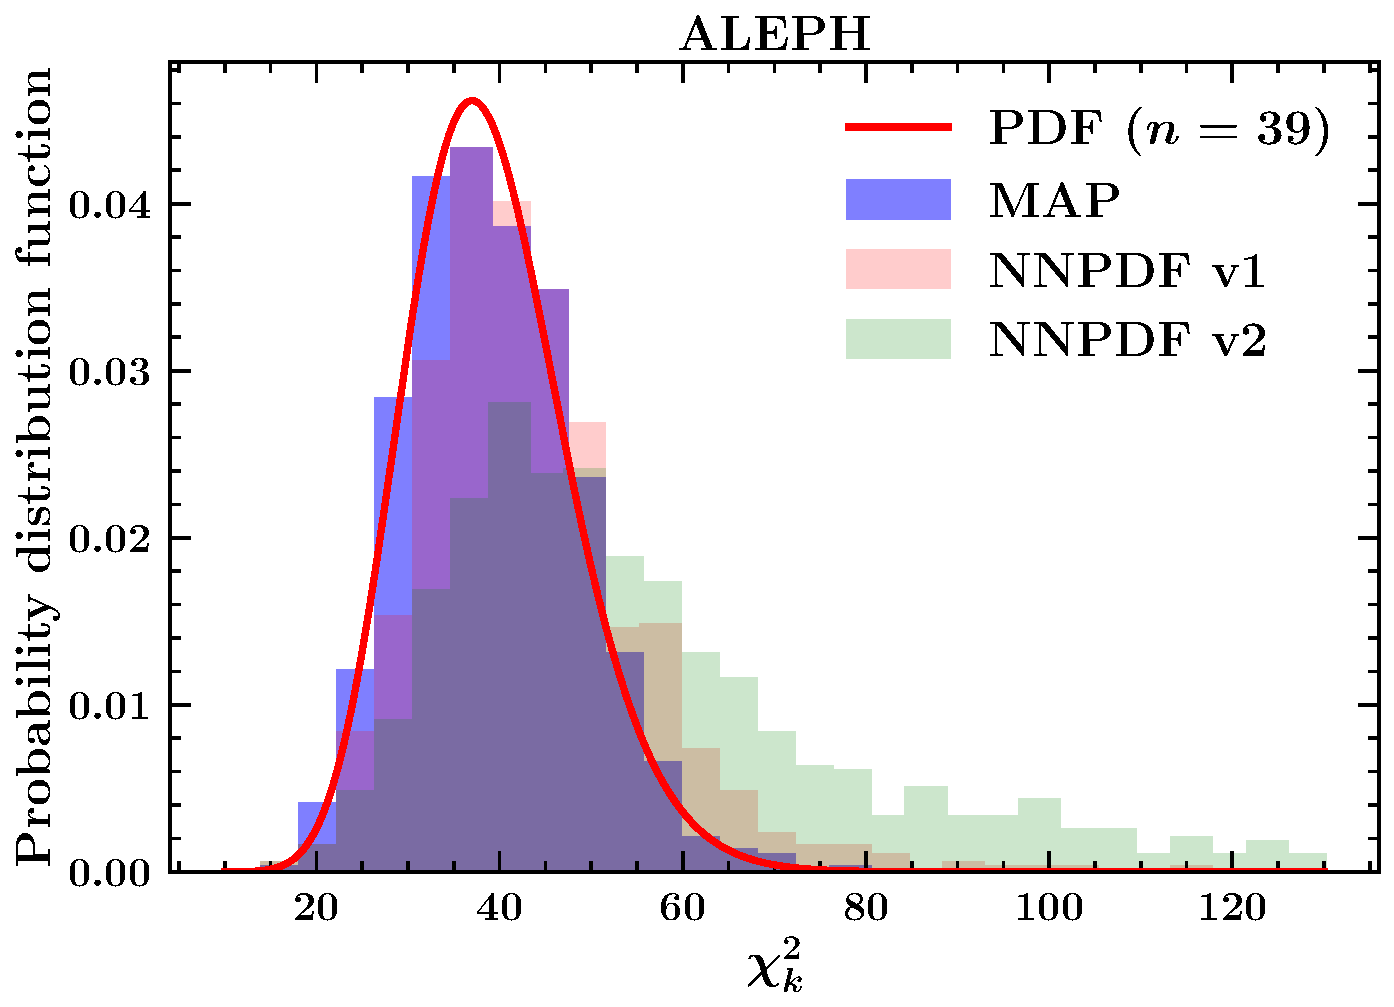
\includegraphics[width=0.49\textwidth]{plots/Chi2DistALEPH.pdf}
    \caption{Distribution of the $\chi^2$'s of the Monte Carlo replica
      w.r.t. to the corresponding central values for BABAR (left) and
      ALEPH (right) experiments compared to the probability
      distribution function with to the appropriate number of degrees
      of freedom given by the number of data points. The blue
      histograms are produced using Eq.~(\ref{eq:deviations}), the red
      histogram is produced using Eq.~(13) of Ref.~\cite{Ball:2008by}
      where multiplicative uncertainties are treated as relative,
      while the green histogram is produced using Eq.~(20) of
      Ref.~\cite{Ball:2014uwa}. \label{fig:Chi2Dist}}
  \end{centering}
\end{figure}

\section{The D'Agostini ``bias''}

The main topic of this section is the so-called D'Agostini ``bias''
(DAB) originally presented in Ref.~\cite{DAgostini:1993arp}. Quoting
from the abstract of that paper: ``Best fits to data which are
affected by systematic uncertainties on the normalisation factor have
the tendency to produce curves lower than expected [...]. This bias
can become unacceptable if the normalisation error is large, or a
large number of data points are used''. In the following, I will
summarise the arguments behind this conclusion. I will then move to
giving my own view on this question arguing that the DAB is in fact
not a bias but rather a feature of correlation uncertainties in
general and not of multiplicative uncertainties in particular. This
implies that the distinction between additive and normalisation
uncertainties is effectively immaterial. Specifically, what really
triggers the DAB is \textit{not} the fact the uncertainty is on the
multiplication factor but rather that it typically gives raise to
correlated uncertainties that are different in \textit{absolute}
size. To show this, below I will show that the DAB takes place also in
the presence of additive uncertainties that are different in absolute
size. Conversely, I will show that the DAB does not takes place when
considering multiplicative uncertainties and the central values are
identical. The bottom line is that any difference in absolute size
between correlated uncertainties causes a deviation from the
expectation according to which the best fit value should be given by
the weighted average of the experimental central values weighted by
the inverse of the squared uncorrelated uncertainties. This deviation
from the expectation is the origin of the DAB.

In order to present the argument, Ref.~\cite{DAgostini:1993arp}
considers a data set made of two data points with the respective
uncorrelated uncertainty, $x_i\pm\sigma_i$ with $i=1,2$. In addition,
it is assumed that $x_i$ measure the same quantity and thus they can
be fitted with a single constant $\mu$. Two cases are treated. In the
first case the two data points are also affected by a single offset
(additive) correlated uncertainty $\sigma_c$. In the second case,
instead, the data points are affected by a normalisation correlated
uncertainty whose size is proportional to the central values through
the factor $\delta_f$. Given the simplicity of the problem, it is
possible in both cases to analytically compute the best value of $\mu$
and its uncertainty $\delta\mu$ by minimising the $\chi^2$ and
computing its second derivative at the minimum. As usual the $\chi^2$
is defined as:
\begin{equation}
\chi^2 = \sum_{i,j=1}^2y_iV^{-1}_{ij}y_j = \mathbf{y}^T\cdot
\mathbf{V}^{-1}\cdot \mathbf{y}\,,
\end{equation}
where $y_i=\mu-x_i$ and $V^{-1}_{ij}$ are the entries of the inverse
of the covariance matrix.

Let us start with the offset case in which the covariance matrix takes
the form:
\begin{equation}
\mathbf{V}=
\begin{pmatrix}
\sigma_1^2+\sigma_c^2& \sigma_c^2\\
\sigma_c^2& \sigma_2^2+\sigma_c^2
\end{pmatrix}\,,
\end{equation}
whose inverse is:
\begin{equation}
\mathbf{V}^{-1}=\frac{1}{D}
\begin{pmatrix}
\sigma_2^2+\sigma_c^2& -\sigma_c^2\\
-\sigma_c^2& \sigma_1^2+\sigma_c^2
\end{pmatrix}\,,
\end{equation}
with $D=\sigma_1^2 \sigma_2^2+(\sigma_1^2+\sigma_2^2)
\sigma_c^2$. With this I can straightforwardly compute the $\chi^2$:
\begin{equation}
\chi^2=\frac{\sigma_2^2y_1^2+\sigma_1^2y_2^2+(y_1-y_2)^2\sigma_c^2}{D}\,,
\end{equation}
that can be minimised w.r.t. to $\mu$ by requiring that:
\begin{equation}
  \left.\frac{d\chi^2}{d\mu}\right|_{\mu=\overline{\mu}} =
  \left.2\frac{\sigma_2^2y_1+\sigma_1^2y_2}{D}\right|_{\mu=\overline{\mu}}=0\,,
\label{eq:minchi2}
\end{equation}
where $\overline{\mu}$ is the best fit value of $\mu$. Notice the
cancellation in the numerator of the correlated uncertainty
$\sigma_c$. This ``accidental'' cancellation in the offset case,
caused by the fact that $\sigma_c$ is the same for both $x_1$ and
$x_2$, can be regarded as the (misleading) evidence that the DAB only
takes place in the normalisation case. The solution to
Eq.~(\ref{eq:minchi2}) is:
\begin{equation}
\overline{\mu} =
\frac{\sigma_2^2x_1+\sigma_1^2x_2}{\sigma_1^2+\sigma_2^2}=\frac{\frac{x_1}{\sigma_1^2}+\frac{x_2}{\sigma_2^2}}{\frac{1}{\sigma_1^2}+\frac{1}{\sigma_2^2}}\,,
\label{eq:offcv}
\end{equation}
that fulfils the intuitive expectation that the best value of $\mu$
should be a weighted average of the central values weighted by the
inverse of the uncorrelated uncertainties squared. One can also compute
the uncertainty of $\overline{\mu}$, $\delta\mu$, by simply computing
the inverse of the second derivative of the $\chi^2$ at
$\mu=\overline{\mu}$:\footnote{Actually, the second derivative of the
  $\chi^2$ does not depend on $\mu$ and thus it is not necessary to
  set $\mu=\overline{\mu}$.}
\begin{equation}
  \delta\mu^2 =
  \left[\frac12\frac{d^2\chi^2}{d\mu^2}\right]_{\mu=\overline{\mu}}^{-1}
  = \frac {\sigma_1^2 \sigma_2^2+(\sigma_1^2+\sigma_2^2)
    \sigma_c^2}{\sigma_2^2+\sigma_1^2}=\frac
  {1+\frac{\sigma_c^2}{\sigma_1^2}+\frac{\sigma_c^2}{\sigma_2^2}
  }{\frac{1}{\sigma_1^2}+\frac{1}{\sigma_2^2}}\,.
\label{eq:offcvunc}
\end{equation}

I now move to considering the normalisation case in which the
covariance matrix reads:
\begin{equation}
\mathbf{V}=
\begin{pmatrix}
\sigma_1^2+\delta_f^2x_1^2& \delta_f^2x_1x_2\\
\delta_f^2x_1x_2& \sigma_2^2+\delta_f^2x_2^2
\end{pmatrix}\,,
\end{equation}
whose inverse is:
\begin{equation}
\mathbf{V}^{-1}=\frac{1}{D}
\begin{pmatrix}
\sigma_2^2+\delta_f^2x_2^2& -\delta_f^2x_1x_2\\
-\delta_f^2x_1x_2& \sigma_1^2+\delta_f^2x_1^2
\end{pmatrix}\,,
\end{equation}
with
$D=\sigma_1^2\sigma_2^2+\delta_f^2(\sigma_1^2x_2^2+\sigma_2^2x_1^2)$. The
resulting $\chi^2$ is:
\begin{equation}
\chi^2=\frac{1}{D}\left[\sigma_2^2y_1^2+ \sigma_1^2y_2^2+\delta_f^2(x_2y_1 -x_1y_2)^2\right]\,.
\end{equation}
The minimum is computed as:
\begin{equation}
  \left.\frac{d\chi^2}{d\mu}\right|_{\mu=\overline{\mu}} = \left.2\frac{\sigma_2^2y_1+ \sigma_1^2y_2+\delta_f^2(x_2 -x_1)(x_2y_1 -x_1y_2)}{D}\right|_{\mu=\overline{\mu}}=0\,.
\end{equation}
This time, differently from the offset case, the correlated
uncertainties in the denominator do not cancel and the result of the
equation above is:
\begin{equation}
\overline{\mu} =
\frac{\sigma_2^2x_1+\sigma_1^2x_2}{\sigma_1^2+\sigma_2^2+(\delta_f
  x_1-\delta_f
  x_2)^2}=\frac{\frac{x_1}{\sigma_1^2}+\frac{x_2}{\sigma_2^2}}{\frac{1}{\sigma_1^2}+\frac{1}{\sigma_2^2}+\left(\frac{\delta_f
      x_1-\delta_f x_2}{\sigma_1\sigma_2}\right)^2}\,,
\label{eq:normcv}
\end{equation}
while:
\begin{equation}
  \delta\mu^2 =
  \left[\frac12\frac{d^2\chi^2}{d\mu^2}\right]_{\mu=\overline{\mu}}^{-1}
  =
  \frac{\sigma_1^2\sigma_2^2+\delta_f^2(\sigma_1^2x_2^2+\sigma_2^2x_1^2)}{\sigma_2^2+
    \sigma_1^2+\delta_f^2(x_1 -x_2)^2}=\frac{1+\frac{\delta_f^2
      x_1^2}{\sigma_1^2}+\frac{\delta_f^2
      x_2^2}{\sigma_2^2}}{\frac{1}{\sigma_1^2}+
    \frac{1}{\sigma_2^2}+\left(\frac{\delta_f x_1 -\delta_f
        x_2}{\sigma_1\sigma_2}\right)^2}\,.
\label{eq:normcvunc}
\end{equation}
According to Ref.~\cite{DAgostini:1993arp}, the term proportional to
$\delta_f$ in the denominator of the r.h.s. of Eq.~(\ref{eq:normcv})
is a source of bias in that it deviates from the intuitive expectation
of Eq.~(\ref{eq:offcv}). Being this additional term positive, it tends
to diminish the best fit value.

I will now show that the additional term in the denominator of
Eq.~(\ref{eq:normcv}) is not a specific feature of normalisation
uncertainties. To show this, I consider the same data set of two data
points but where the data point $x_1$ is affected by the additive
uncertainty $\sigma_{c,1}$ and the point $x_2$ by the additive
uncertainty $\sigma_{c,2}$. According to the same procedure followed
above the final result for best-fit value and uncertainty of $\mu$ is:
\begin{equation}
\overline{\mu} =
\frac{\frac{x_1}{\sigma_1^2}+\frac{x_2}{\sigma_2^2}}{\frac{1}{\sigma_1^2}+\frac{1}{\sigma_2^2}+\left(\frac{\sigma_{c,1}-\sigma_{c,2}}{\sigma_1\sigma_2}\right)^2}\,,
\label{eq:add2cv}
\end{equation}
and:
\begin{equation}
  \delta\mu^2=\frac{1+\frac{\sigma_{c,1}^2}{\sigma_1^2}+\frac{\sigma_{c,2}^2}{\sigma_2^2}}{\frac{1}{\sigma_1^2}+ \frac{1}{\sigma_2^2}+\left(\frac{\sigma_{c,1} -\sigma_{c,2}}{\sigma_1\sigma_2}\right)^2}\,.
\end{equation}
These equations are (somewhat expectedly) equal to
Eqs.~(\ref{eq:normcv}) and~(\ref{eq:normcvunc}) with the only
difference that $\delta_fx_i$ is replaced by
$\sigma_{c,i}$. Therefore, the DAB shows up also when additive
uncertainties are considered as long as they are different in absolute
value. Therefore, the DAB is not a prerogative of normalisation
uncertainties only. As expected, the equations above reduce to
Eqs.~(\ref{eq:offcv}) and~(\ref{eq:offcvunc}) when
$\sigma_{c,1}=\sigma_{c,2}=\sigma_{c}$.

Another important aspect of Eqs.~(\ref{eq:normcv})
and~(\ref{eq:normcvunc}) is that the term that causes the ``bias'' is
proportional to the difference $x_1-x_2$. Therefore, if the central
values happen to be the same that term vanishes and thus no bias is
present. This observation, along with the fact that the DAB is
potentially present also when additive uncertainties are considered,
leads to a simple conclusion: the DAB is present in all cases whenever
there are correlated uncertainties different in absolute value. This
is trivially the case when one introduces different correlated
additive uncertainties, $\sigma_{c,1}$ and $\sigma_{c,2}$ with
$\sigma_{c,1}\neq \sigma_{c,2}$. But this also the case in the
presence of a normalisation uncertainties when central values are
different ($x_1\neq x_2$). On the contrary, if
$\sigma_{c,1}= \sigma_{c,2}$ in the additive case or $x_1=x_2$ in the
multiplicative case, no ``bias'' is present. The conclusion is that
the very distinction between additive and multiplicative uncertainties
is immaterial.

Now that I have established that the DAB is not a prerogative of
normalisation uncertainties only, I will argue that this is in fact
not a bias but a manifestation of large correlated uncertainties in
general that indicates an intrinsic inconsistency of the data set
being considered. I start by observing that, in the presence of
correlations, a visual comparison between data and best fit value is
meaningful only when including the systematic shifts introduces in
Sect.~\ref{eq:sysshifts}. The task is particularly simple due to the
small number of points and the fact that there one single correlated
uncertainty. In particular, there is a single nuisance parameter that
in the normalisation case is given by:
\begin{equation}
\lambda=\frac{\frac{\delta_f x_1^2}{\sigma_1^2}+\frac{\delta_f x_2^2}{\sigma_2^2}}{1+\frac{\delta_f^2 x_1^2}{\sigma_1^2}+\frac{\delta_f^2 x_2^2}{\sigma_2^2}}-\overline{\mu}\frac{\frac{\delta_f x_1}{\sigma_1^2}+\frac{\delta_f x_2}{\sigma_2^2}}{1+\frac{\delta_f^2 x_1^2}{\sigma_1^2}+\frac{\delta_f^2 x_2^2}{\sigma_2^2}}\,.
\end{equation}
It is the quantity:
\begin{equation}
\hat{\mu}_i =\overline{\mu}+\lambda \delta_fx_i\,,
\label{eq:shiftedvals}
\end{equation}
that can be directly compared to the data-point central
values. Unfortunately, the analytic form of this quantity is not very
informative but to see the effect of the systematic shifts I consider
the very same example given in the introduction of
Ref.~\cite{DAgostini:1993arp}, \textit{i.e.} a data set of two
measurements: $8.0\pm 2\%$ and $8.5\pm 2\%$ having a common 10\%
normalisation uncertainty.

\begin{figure}[h]
  \begin{centering}
    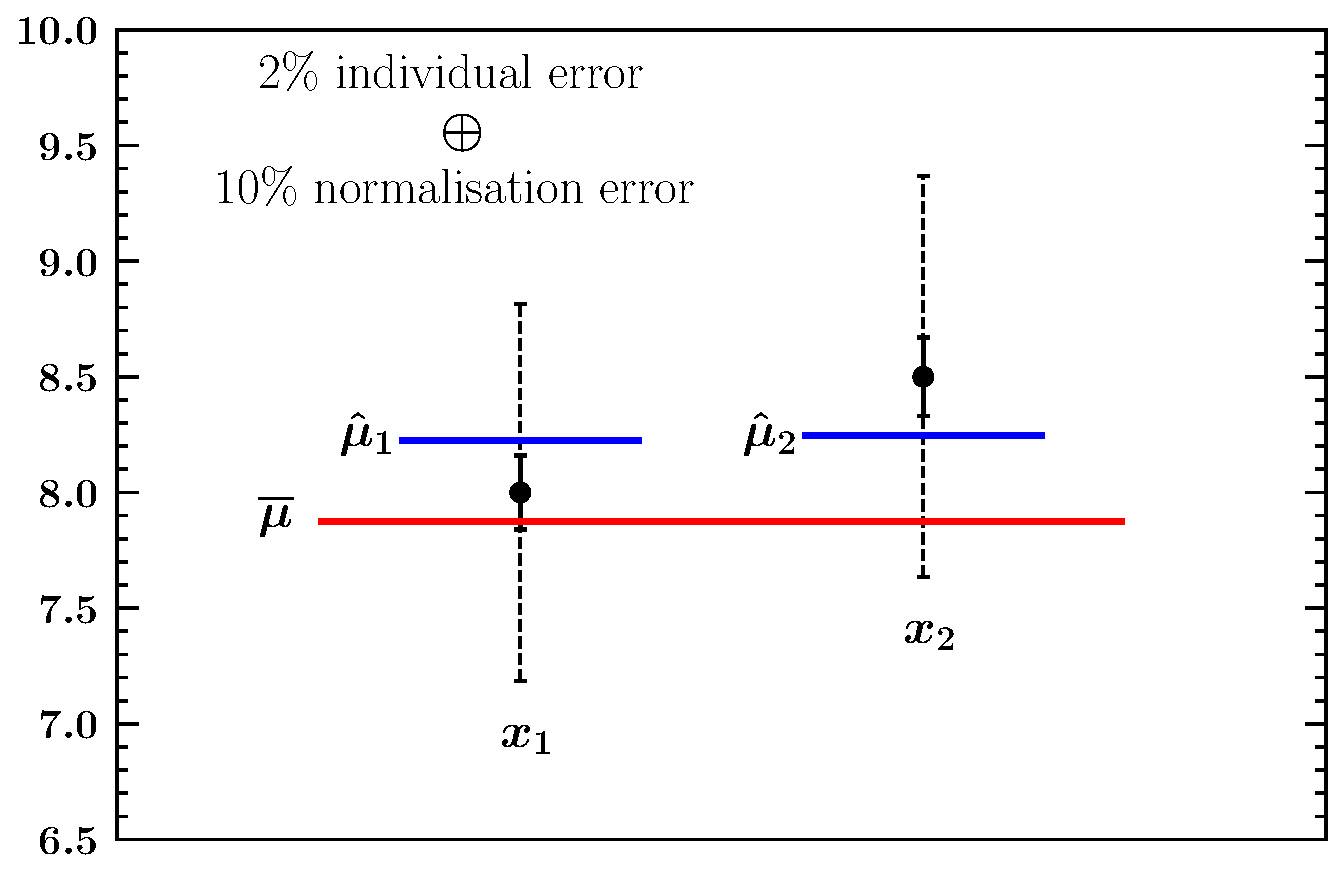
\includegraphics[width=0.7\textwidth]{plots/DAgostiniExample.pdf}
    \caption{Numerical example taken from
      Ref.~\cite{DAgostini:1993arp} of a data set of two points with
      central value 8.0 and 8.5 (black points) each affected by a 2\%
      uncorrelated uncertainty (solid error bars) and a common 10\%
      normalisation uncertainty (the dashed error bars indicate the
      sum in quadrature of correlated and uncorrelated
      uncertainties). The horizontal red line corresponds to the best
      fit value given in Eq.~(\ref{eq:offcv}) while the horizontal
      blue lines correspond to the shifted values according to
      Eq.~(\ref{eq:shiftedvals}).\label{fig:DAgostiniExample}}
  \end{centering}
\end{figure}
Fig.~\ref{fig:DAgostiniExample} shows the result of minimising the
$\chi^2$ to determine the best fit value of the parameter $\mu$. The
solid error bars display the uncorrelated uncertainties while the
dashed error bars display the sum in quadrature of correlated and
uncorrelated uncertainties. The best fit value $\overline{\mu}$,
Eq.~(\ref{eq:offcv}), is represented by the horizontal red line. As
argued in Fig.~\ref{fig:DAgostiniExample}, this line lies below both
the central experimental values ($\overline{\mu}\simeq 7.87$)
contradicting the common expectation that best fit value should be
somewhere between the experimental central values. However, as
explained above, a visual comparison in the presence of (large)
correlations is meaningful only when including the systematic
shifts. The inclusion of the shifts yields the two horizontal blue
lines in Fig.~\ref{fig:DAgostiniExample}. The shifted values are
$\hat{\mu}_1 \simeq 8.22$ and $\hat{\mu}_2 \simeq 8.25$ that indeed
fulfil the common expectation. It is worth noticing that the best fit
$\chi^2$ per degree of freedom is around 4.4, signifying that the
measurements, that are assumed to refer to the same quantity, are in
strong tension. This is a first suggestion that that there is no
problem with the standard inclusion of correlated normalisation
uncertainties in the covariance matrix while the problem seems to be
in the data set.

One may ask what is the meaning of a value of $\overline{\mu}$ that
can be smaller than both $x_1$ and $x_2$ or in general far from both
of them. To answer this question I first observe that, according to
Eq.~(\ref{eq:offcv}), $\overline{\mu}$ tends to zero as the
uncorrelated uncertainties $\sigma_1$ and $\sigma_2$ tend to zero.
This can be seen more explicitly by setting
$\sigma_1=\sigma_2=\varepsilon$ and expanding the $\chi^2$ around
$\varepsilon = 0$:
\begin{equation}
\chi^2\rightarrow
\frac{\mu^2(x_1-x_2)^2}{\varepsilon^2(x_1^2+x_2^2)}+\frac{\left[\mu(x_1+x_2)-(x_1^2+x_2^2)\right]^2}{\delta_f^2
  (x_1^2+ x_2^2)^2}+\mathcal{O}(\varepsilon^2)\,.
\label{eq:chi2exp}
\end{equation}
Therefore, if $x_1\neq x_2$, for $\varepsilon\rightarrow 0$ the
dominant term is the first one and the minimum of the $\chi^2$ in this
limit is clearly at $\mu=0$. If $x_1 = x_2=x$, instead, the first term
drops and the best fit value of the parameter $\mu$ is determined by
the second term that has its minimum at $\mu=x$.

This can be interpreted as follows: as $\sigma_1$ and $\sigma_2$ tend
to zero, the covariance matrix tends to become singular signifying
that $x_1$ and $x_2$ are no longer independent. However, if
$x_1=x_2=x$ the singularity cancels. This is due to the fact that,
without uncorrelated uncertainties, the number of points of the data
set effectively reduces to one. As a matter of fact, in this case
$\varepsilon$ can safely be set to zero and the $\chi^2$ becomes:
\begin{equation}
\chi^2= \left(\frac{\mu - x}{\delta_f  x}\right)^2\,,
\end{equation}
that is evidently the $\chi^2$ associated to one single data point
with central value $x$ and uncertainty $\delta_f x$.\footnote{Note
  that in the case of one-point data set there is no meaning in
  talking about correlated uncertainties. Therefore, $\delta_f x$
  plays the role of an uncorrelated uncertainty.}  As a consequence,
the best fit value of the parameters $\mu$ is simply given by $x$, as
one would expect.

If $x_1\neq x_2$, instead, the singularity of the covariance matrix
does not cancel and the first term in Eq.~(\ref{eq:chi2exp}) dominates
in the limit $\varepsilon\rightarrow0$. This is a situation in which
two totally dependent measurements of the same quantity have different
central values. It is thus to be expected that the $\chi^2$ becomes
arbitrarily large because the two data points are inconsistent and
thus impossible to be simultaneously fitted. In this situation, the
parameter $\mu$ attempts to minimise the $\chi^2$ by tending to
zero. More specifically, when correlations dominate over uncorrelated
uncertainties, the $\chi^2$ is proportional to (the square of) the
cross difference $\delta_fx_1y_2-\delta_fx_2y_1$,\footnote{In general,
  this can be seen as $\sigma_{c,1}y_2-\sigma_{c,2}y_1$.}  with
$y_i = \mu - x_i$. Therefore, if $x_1\neq x_2$, this difference is
minimal when $y_i\simeq x_i$ which is equivalent to $\mu\simeq 0$. It
is also interesting to observe that the first term in
Eq.~(\ref{eq:chi2exp}) does not depend of $\delta_f$. Therefore, the
size of the $\chi^2$ is entirely driven by the difference $x_1-x_2$,
no matter the precise value of normalisation uncertainty.

In conclusion, it appears that data sets dominated by normalisation
(or equivalently widely spread correlated) uncertainties carry an
intrinsic degree of inconsistency that, when attempting to fit them,
manifests into the DAB. Therefore, from this point of view, the DAB is
not a flaw of the fitting procedure but rather an indication that the
data set is intrinsically inconsistent. It thus appears
counterproductive, if not wrong, to adjust the definition of the
$\chi^2$ to accommodate an inconsistency of the data set.

\subsection{The effect of the $t_0$ prescription}

In this section, I consider the effect of the iterative $t_0$
prescription on the best fit value $\overline{\mu}$. The $t_0$
prescription essentially replaces the normalisation uncertainties
$\delta_fx_1$ and $\delta_fx_2$ with one single correlated
uncertainties $\delta_f t_0$, where $t_0$ is a ``guess'' for
$\mu$. The net effect of this replacement is that the terms
$\delta_fx_1$ and $\delta_fx_2$ in the r.h.s. of both
Eqs.~(\ref{eq:normcv}) and~(\ref{eq:normcvunc}) are replaced by
$\delta_ft_0$ and thus cancel, reducing to Eqs.(\ref{eq:offcv})
and~(\ref{eq:offcvunc}). But this should not be surprising because the
$t_0$ prescription is essentially replacing two correlated
uncertainties that are different in value with two correlated
uncertainties that are instead \textit{equal}. This makes the
normalisation case artificially equal to the offset case in which the
DAB is not present.

Now, what happens if one iterates the $t_0$? Let us indicate with
$\overline{\mu}_i$ and $\delta\mu_i^2$ best fit value and variance at
the $i$-th iteration. As explained above, the zero-th iteration gives:
\begin{equation}
\overline{\mu}_0 =\frac{\frac{x_1}{\sigma_1^2}+\frac{x_2}{\sigma_2^2}}{\frac{1}{\sigma_1^2}+\frac{1}{\sigma_2^2}}\,,
\end{equation}
and:
\begin{equation}
  \delta\mu_0^2 = \frac{1+\frac{\delta_f^2 t_0^2}{\sigma_1^2}+\frac{\delta_f^2 t_0^2}{\sigma_2^2}}{\frac{1}{\sigma_1^2}+ \frac{1}{\sigma_2^2}}\,.
\end{equation}
Since $\overline{\mu}_0$ does not depend on $t_0$, all following
iterations will give the exact same result, \textit{i.e.}
$\overline{\mu}_i=\overline{\mu}_0$ $\forall i>0$. The stabilisation
happens only one step further for the uncertainty for which one finds
$\delta\mu_i^2=\delta\mu_1^2$ $\forall i>1$, with:
\begin{equation}
  \delta\mu_1^2 = \frac{1+\frac{\delta_f^2 \overline{\mu}_0^2}{\sigma_1^2}+\frac{\delta_f^2 \overline{\mu}_0^2}{\sigma_2^2}}{\frac{1}{\sigma_1^2}+ \frac{1}{\sigma_2^2}}=\frac{1}{\frac{1}{\sigma_1^2}+ \frac{1}{\sigma_2^2}}+\delta_f^2\overline{\mu}_0^2\,.
\end{equation}
As above, I set $\sigma_1=\sigma_2=\varepsilon$ getting:
\begin{equation}
\overline{\mu}_0 =\frac{x_1+x_2}{2}\,,
\end{equation}
and:
\begin{equation}
  \delta\mu_1^2 = \frac{\varepsilon^2}{2}+\frac{\delta_f^2  (x_1+x_2)^2}{4}\,.
\end{equation}
Now, I plug $\overline{\mu}_0$ into the original definition of the
$\chi^2$. The result is:
\begin{equation}
\chi^2=\left(\frac{x_1- x_2}{2}\right)^2\left[\frac{1}{\varepsilon^2+\delta_f^2(x_1^2+x_2^2)}+\frac{1}{\varepsilon^2}\right]\,.
\end{equation}

\newpage
\bibliographystyle{ieeetr}
\bibliography{bibliography}

\end{document}
